\documentclass{beamer}       % print frames
%\documentclass[notes=only]{beamer}   % only notes
%\documentclass{beamer}              % only frames
\newcounter{savedenum}
\newcommand*{\saveenum}{\setcounter{savedenum}{\theenumi}}
\newcommand*{\resume}{\setcounter{enumi}{\thesavedenum}}
\usepackage{multienum}
\usepackage[T1]{fontenc}
\usepackage{minted}
\usepackage{upquote}
\AtBeginDocument{%
\def\PYZsq{\textquotesingle}%
}
\usepackage[notocbib]{apacite}
    \renewcommand{\APACrefatitle}[2]{#1}
    \renewcommand{\APACrefbtitle}[2]{#1}
    \renewcommand{\APACrefbtitle}[2]{\Bem{#1}}
    \renewcommand{\APACrefaetitle}[2]{[#2]}
    \renewcommand{\APACrefbetitle}[2]{[#2]} 
\usepackage{textpos}
\usepackage{setspace}
\usefonttheme{serif}
%\usepackage{graphicx}
\usetheme{Boadilla}
\usepackage{hyperref}
\usepackage[UKenglish]{babel}
\usepackage{multicol}
\setcounter{tocdepth}{1} 
\usecolortheme{orchid}
\title[FEAST]{Shifting discourse-semantics of risk in US newspapers, 1987--2014}
\author[McDonald \& Zinn]{Daniel McDonald \and Jens Zinn~\\~\\\texttt{@interro\_gator}~\\~\\This slideshow is available at: \url{http://git.io/vBfbw}~\\~\\}

\date{\today}

\begin{document}

\addtobeamertemplate{frametitle}{}{%
\begin{textblock*}{100mm}(.775\textwidth,-.5cm)

\includegraphics[scale=.235]{../../images/unimelblong}
\end{textblock*}}

\frame{\titlepage}


\begin{frame}
    \frametitle{Overview}
    
    \begin{itemize}
    \item Context of the investigation: risk theory
    \item Data and research questions
    \item Linguistic approaches to risk
    \item Our methods and linguistic findings
    \item Sociological significance of the results
    \end{itemize}

    ~\\ This slideshow is available at: \url{http://git.io/vBfbw}

\end{frame}

\begin{frame}\frametitle{The project(s)}

I'm presenting work from closely related projects:

\begin{enumerate}
    \item Risk words in the NYT, 1963, 1987--2014
    \item Risk words in NYT health articles
    \item Risk words in six US newspapers, 1987--2014
\end{enumerate}

All investigations involve making longitudinally structured, parsed corpora and looking at how risk words behave.

\end{frame}

\begin{frame}
    \frametitle{Context: sociological risk theory}
    
    From previous sociological and linguistic research, we know that:

    \begin{itemize}
    \item Risk as concept is sociologically important
    \begin{itemize}
        \item New global risks \cite{beck_risk_1992}
        \item Calculative technologies \cite{dean_governmentality:_1999}
        \item Individualisation (Beck) and Technologies of the Self \cite{dean_risk_1998}
        \item Risk-taking \cite{luhmann_risk:_1993}
    \end{itemize}
    \item Risk as lexical item is increasingly frequent in print journalism (Zinn 2011)
    \item Risk as a lexical item in naturalistic text may behave contrary to expectations \cite{hamilton_meanings_2007}
    \end{itemize}
\end{frame}

\begin{frame}
    \frametitle{The data}

    \begin{enumerate}
        \item \emph{NYT Annotated Corpus}: 1.8 million articles, 1987--2007 \cite{sandhaus_new_2008}
        \item \emph{ProQuest Newsstand} for NYT 2007--2014
        \item \emph{ProQuest Newsstand} for five other newspapers, 1987--2014
        \begin{enumerate}
            \item \emph{Washington Post}
            \item \emph{Tampa Bay Times}
            \item \emph{USA Today}
            \item \emph{Chicago Tribune}
            \item \emph{Wall Street Journal}
        \end{enumerate}
    \end{enumerate}
\end{frame}

\begin{frame}
    \frametitle{Research questions}

    \begin{itemize}
        \item What are risk words doing in the NYT?
        \item How has the behaviour of risk words changed in the NYT between 1963 and 2014?
        \item Can we connect these findings to sociological theories of risk?
        \item What kinds of tools and methods can we use\slash develop to do this kind of research?
    \end{itemize}
\end{frame}

\begin{frame}
    \frametitle{New methodologies}

    New kinds of data and tools make it possible to empirically analyse risk language in new ways:
    
    \begin{itemize}
    \item Digitisation of newspapers means we have large, well-structured datasets
    \item Automatic annotation of text makes it possible to search for lexical and grammatical features in tandem
    \item Modern programming languages facilitate:
    \begin{itemize}
        \item Automation
        \item Reproducibility
        \item Transparency
    \end{itemize}
    \end{itemize}

\end{frame}

\begin{frame}
    \frametitle{Frame semantic approach}

    Frame semantics: risk as a cognitive schema \cite{fillmore_toward_1992}

\begin{itemize}
    \item Conceptualises risk mostly as experiential Process\slash Event
    \begin{itemize}
        \item \emph{What kind of participants and circumstances occur when risk is the Process?}
    \end{itemize}
    \item Problem: risk often takes less prominent experiential roles
    \begin{itemize}
        \item Is the risk frame actually invoked when the word is used?
        \item Example:
    \end{itemize}
    \end{itemize}

    ~\\
    \footnotesize
    \begin{quote}
    \noindent
    \texttt{Mr. Tepfer noted that Mr. Douglas, who was in the neighborhood when the body was found and was interviewed by the police at the time, `preyed on \textbf{at-risk women}, on prostitutes, and he engaged in sex and strangled them to death.' }
    \end{quote}

\end{frame}

\begin{frame}
    \frametitle{The risk frame}
    \centering
    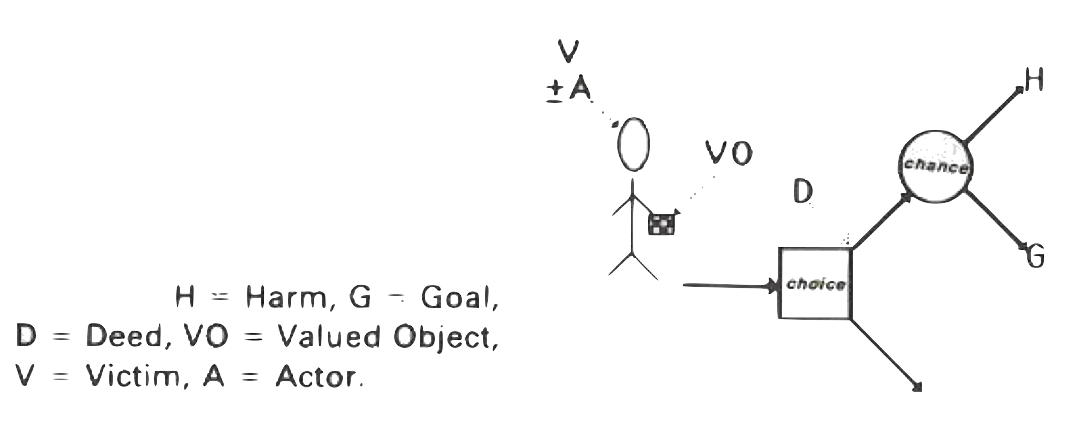
\includegraphics[width=0.90\textwidth]{../../images/riskframe.png}
\end{frame}


\begin{frame}
    \frametitle{Corpus linguistic approach}

    Corpus linguistics: risk as token \cite{hamilton_meanings_2007}

    \begin{itemize}
    \item Topics and text-types in which risk tokens appear
    \item Collocates of risk tokens
    \item Risk appears a lot in discussions of health
    \item Use of risk words is different to invented examples
    \end{itemize}

    Shortcomings:

    \begin{itemize}
        \item Smaller corpus size, heterogeneity of samples
        \item No parsing, lemmatisation
        \item No systematic connection of lexicogrammatical patterns to discourse\slash meaning
    \end{itemize}

\end{frame}

\begin{frame}
    \frametitle{Our methods}
    
    \begin{itemize}
    \item Get all paragraphs containing \texttt{\textbackslash brisk} in all 1987--mid 2014 articles
    \item Annotate\slash parse the data with full \emph{Stanford CoreNLP} suite
    \item Develop \texttt{corpkit}, a toolkit for manipulating the corpus and communicating results
    \item Interrogate the corpus according to notions from systemic functional grammar
    \item Connect to sociological theory
    \end{itemize}
\end{frame}

\begin{frame}
\frametitle{SFL: Introduction}
\begin{itemize}
\item \emph{Systemic}: focus on relationships between signs in the sign-system
\item \emph{Functional}: focus on language as a tool for the performance of functions
\begin{enumerate}
    \item Interpersonal: negotiating relationships
    \item \textbf{Experiential: representing the world}
    \item Textual: reflexive organisation into meaninful sequences
\end{enumerate}
In general, print news in a single publication is fairly stable in terms of interpersonal and textual features.
\end{itemize}

\end{frame}

\begin{frame}
    \frametitle{Overview of SFL}
    \centering
    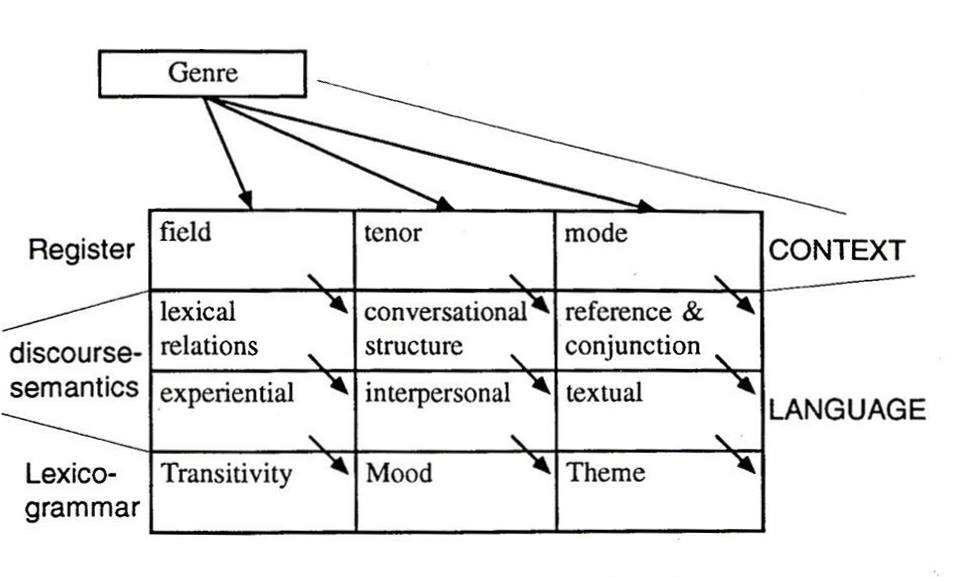
\includegraphics[width=0.90\textwidth]{../../images/egginsfixed.jpg}
\end{frame}

\begin{frame}\frametitle{Transitivity system}
\begin{itemize}
    \item Focus on the clause as a unit of analysis
    \item Centre on the \emph{process} (i.e. rightmost verb in VP)
    \item Processes \emph{select} participants (i.e. arguments of the verb)
    \item PPs and RBs are typically \emph{circumstances}
\end{itemize}
\end{frame}

\begin{frame}
    \frametitle{Constituency grammar}
    \centering
    \includegraphics[width=0.67\textwidth]{../../images/const-grammar}
\end{frame}

\begin{frame}
    \frametitle{Dependency grammar}
    \centering
    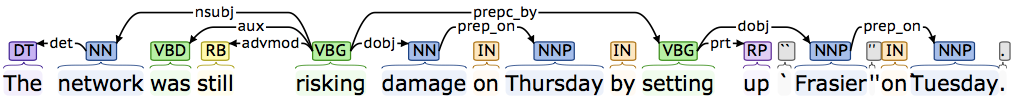
\includegraphics[width=0.99\textwidth]{../../images/depparse}
\end{frame}

\begin{frame}\frametitle{The controversial question}

The question: \emph{Can we get systemic functional information from constituency and dependency parses?}

~\\~\\~\\~\\

The answer: \emph{Yep, quite a lot.}
\end{frame}


\begin{frame}\frametitle{Developing tools}
How to investigate this huge dataset, and make the investigation transparent\slash reproducible?

\begin{itemize}
    \item \texttt{corpkit}: a Python module designed for parsed and structured corpora, with some systemic functional awareness
    \begin{itemize}
        \item \texttt{interrogator()}: search for lexicogrammatical phenomena in each subcorpus, tally results, output Pandas objects
        \item \texttt{editor()}: edit results, calculate keyness, linear regression 
        \item \texttt{plotter()}: visualise via \emph{matplotlib} 
        \item \texttt{conc()}: concordance via parses 
    \end{itemize}
    \item Sciptable, multiprocessing, handles arbitrary data, open-source
    \item More recently, a GUI, aimed at corpus linguists
\end{itemize}
\end{frame}

\begin{frame}
    \frametitle{\texttt{corpkit}: GUI}
    \centering
    \includegraphics[width=0.95\textwidth]{../../images/interrogate}
\end{frame}

\begin{frame}
    \frametitle{\texttt{corpkit}: concordancer}
    \centering
    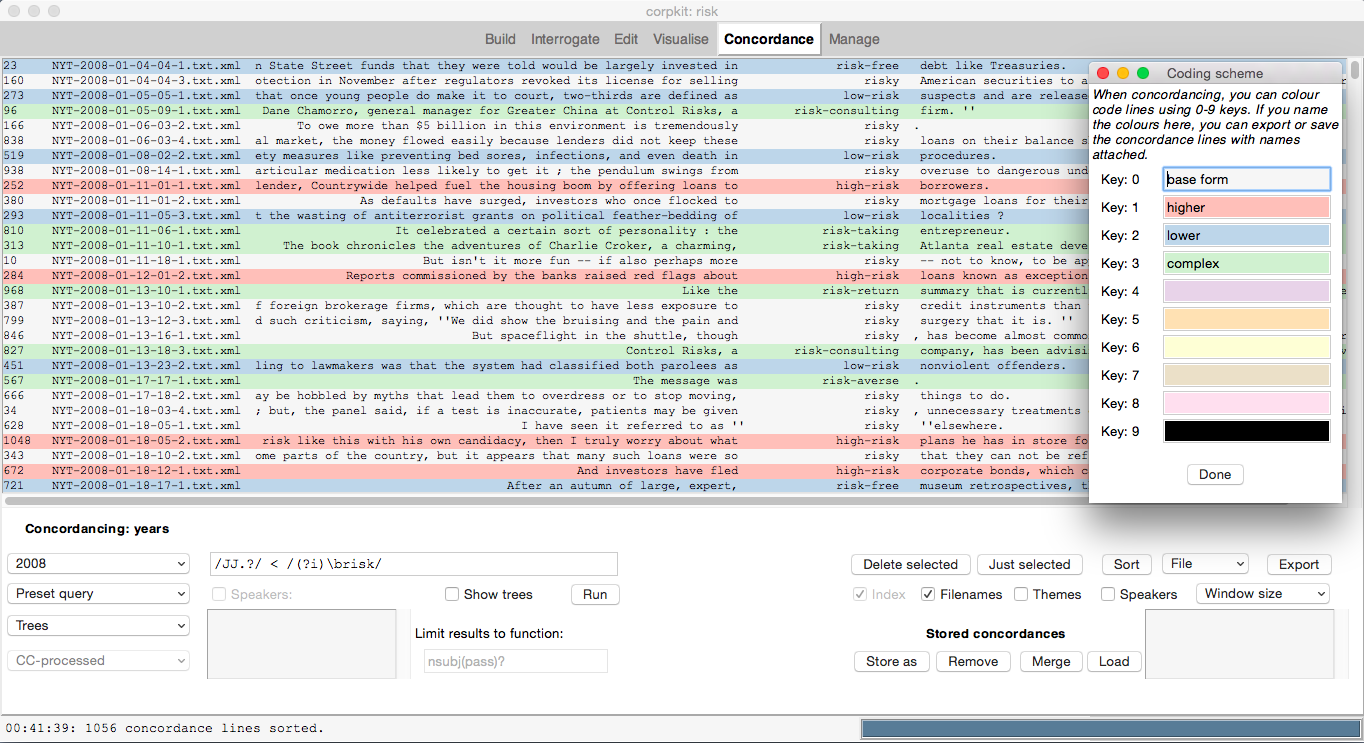
\includegraphics[width=0.95\textwidth]{../../images/conc2}
\end{frame}

\begin{frame}
    \frametitle{\texttt{corpkit}: plotting}
    \centering
    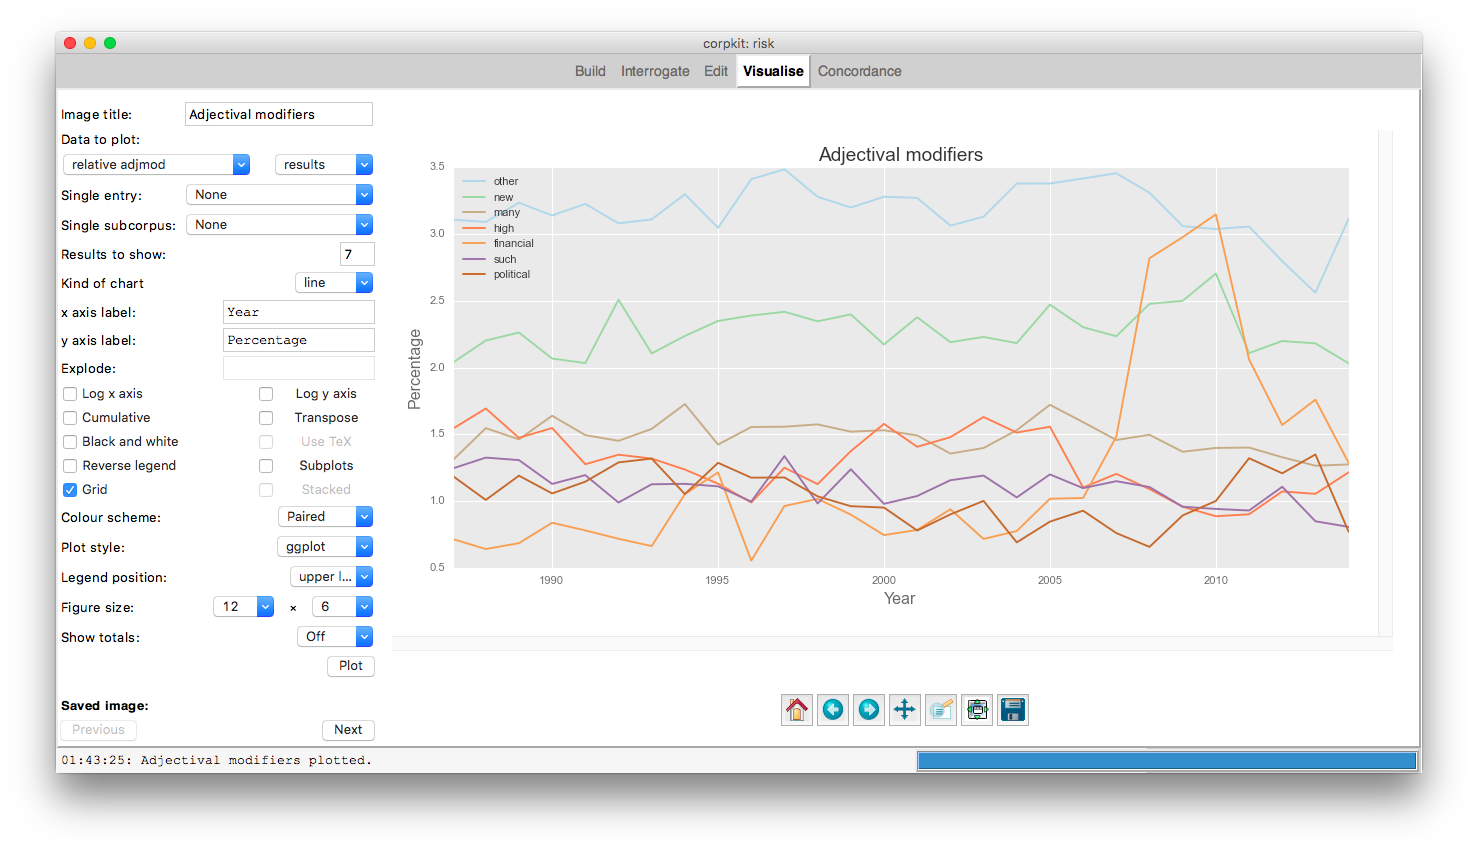
\includegraphics[width=0.95\textwidth]{../../images/plott}
\end{frame}


\begin{frame}[fragile]
\frametitle{\texttt{corpkit}: Example code}

\begin{minted}[fontsize=\normalsize,linenos=true]{python}
# import module and set data path
>>> from corpkit import *
>>> corpus = 'data/NYT-parsed'

# get pos of risk words, show word class
>>> res = interrogator(corpus, 'words', r'\brisk', 
...    show = ['p'], lemmatise = True)

# get relative frequency
>>> rel = editor(res.results, '%', res.totals, keep_top = 4)

# visualise
>>> plotter('Word class of risk words', rel.results, 
...    kind = 'area', style = 'seaborn-talk')
\end{minted}
\end{frame}

\begin{frame}
    \frametitle{Example output}
    \centering
    \includegraphics[width=0.90\textwidth]{../../images/pos_sb}
\end{frame}

\begin{frame}
\frametitle{Initial investigation: NYT}

Our first investigation was of the NYT only:

\end{frame}

\begin{frame}
    \frametitle{Nominalisation of risk}
    \centering
    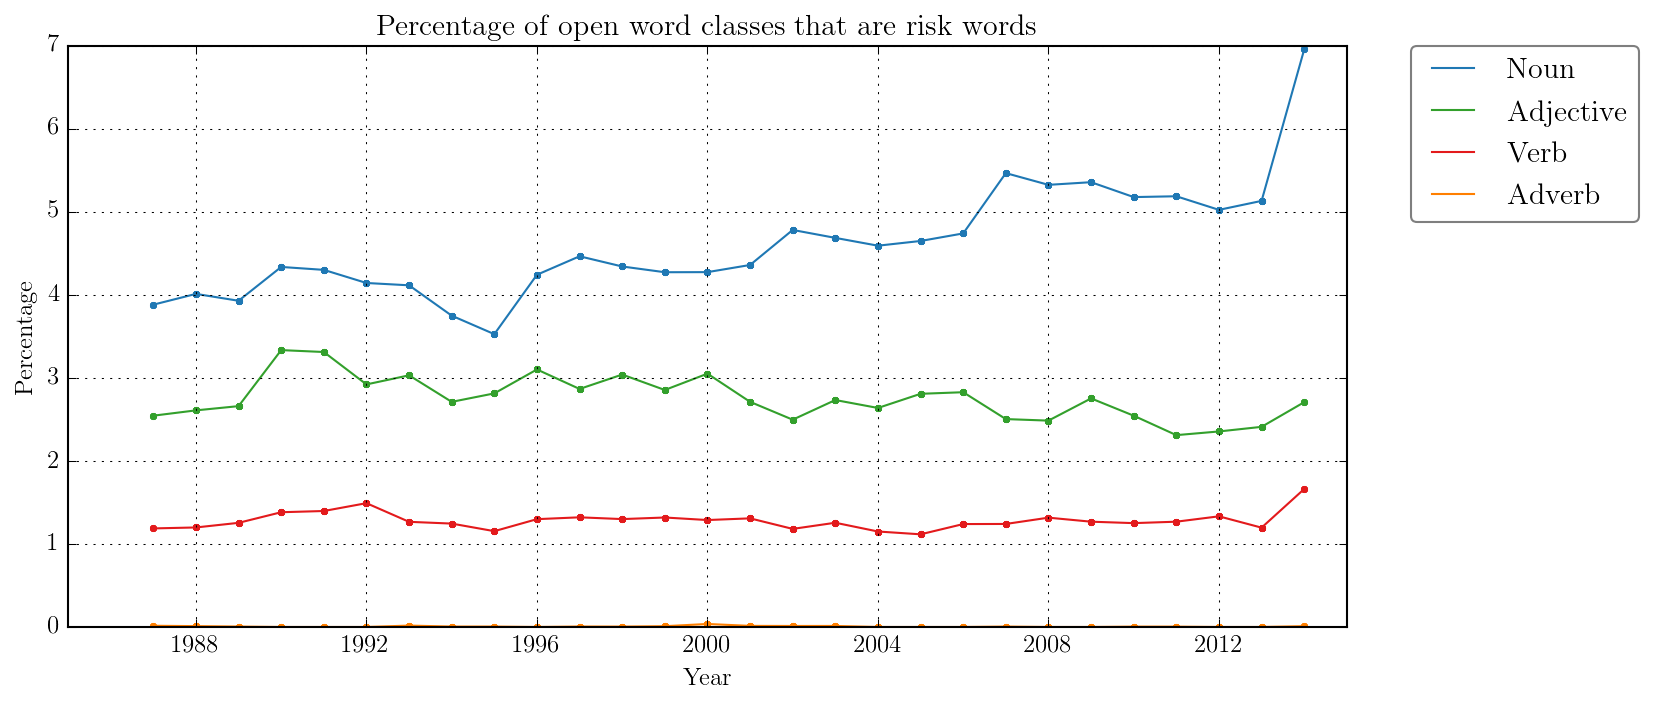
\includegraphics[width=0.99\textwidth]{../../images/percentage-of-open-word-classes-that-are-risk-words}
\end{frame}

\begin{frame}
    \frametitle{Experiential roles of risk words}
    \centering
    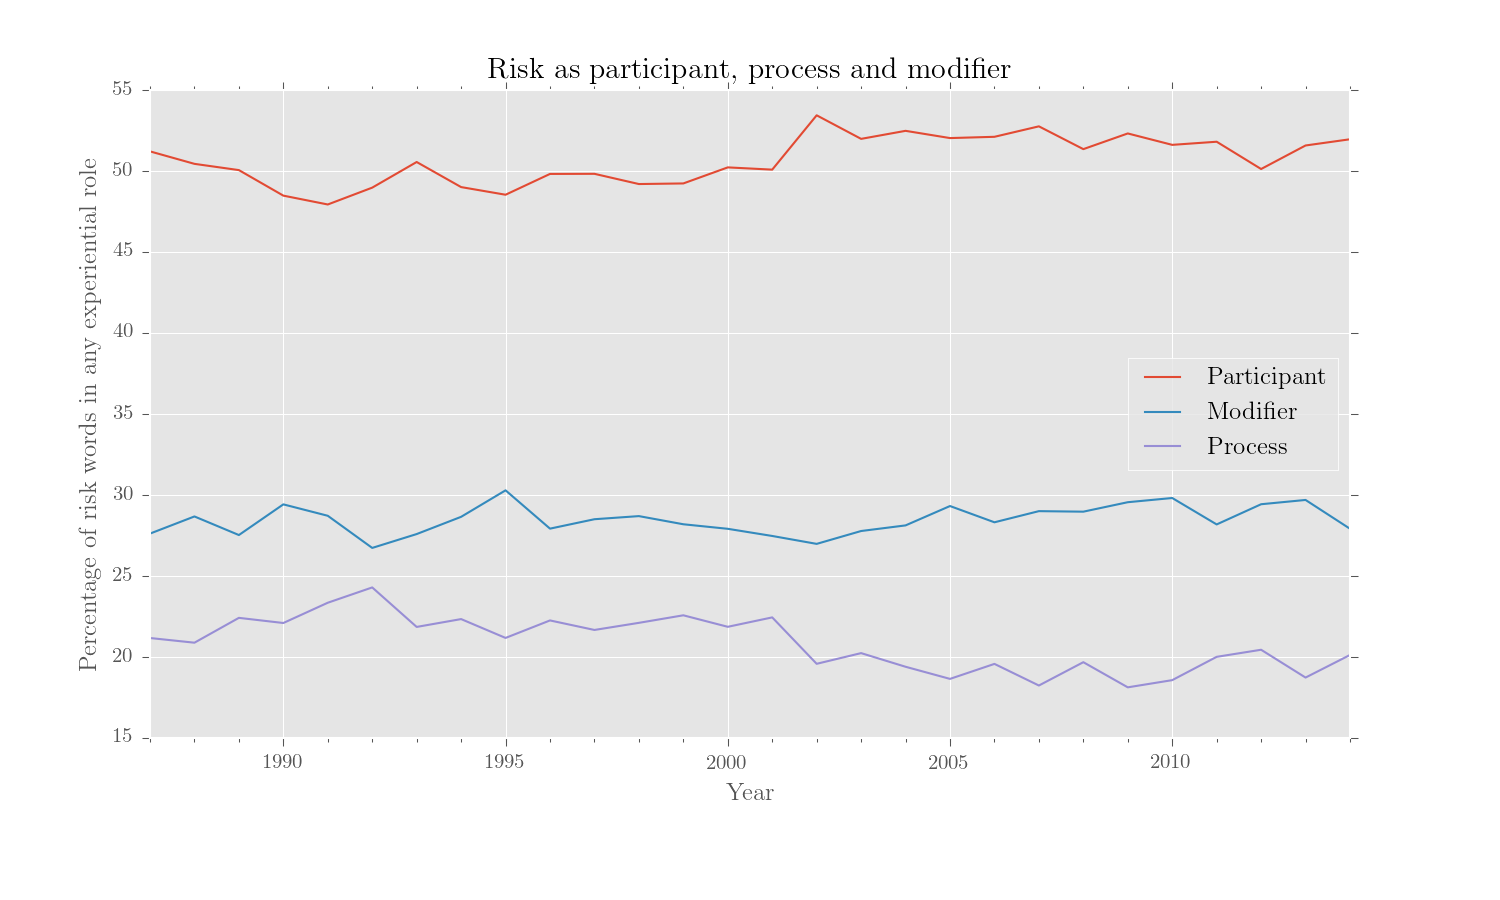
\includegraphics[width=0.99\textwidth]{../../images/ppm_final_colour}

    \noindent \emph{They risked their life} $\rightarrow$ \emph{It was a risk}
\end{frame}

\begin{frame}
    \frametitle{Risk as modifier}
    \centering
    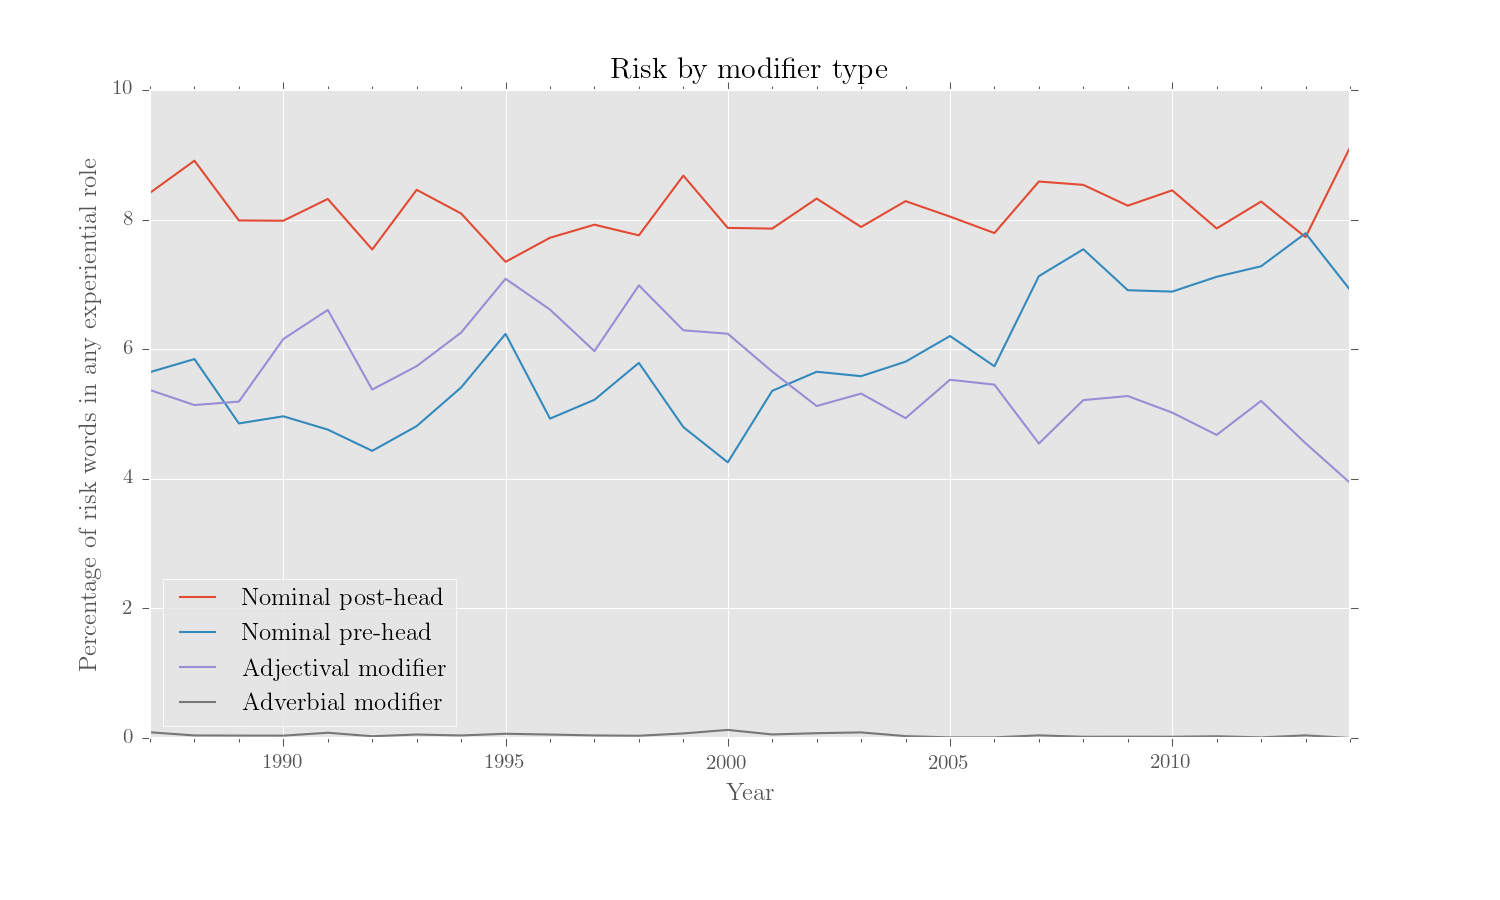
\includegraphics[width=0.99\textwidth]{../../images/risk_by_mod_type_colour}

    \noindent \emph{Risky decision} $\rightarrow$ \emph{risk assessment}
\end{frame}

\begin{frame}
    \frametitle{Risk and power}
    \centering
    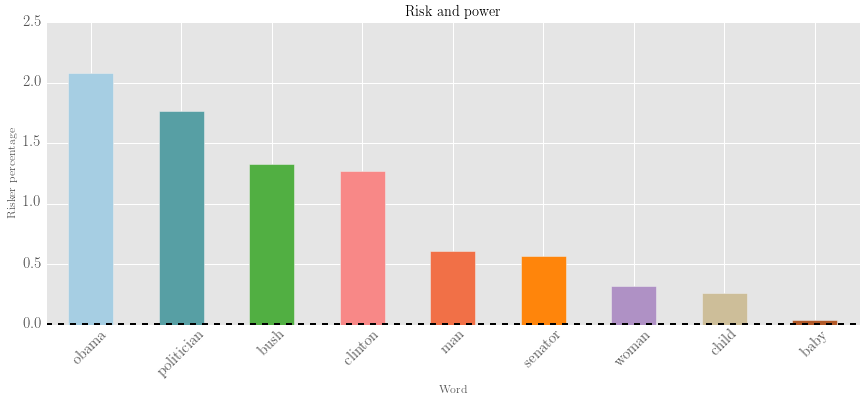
\includegraphics[width=0.99\textwidth]{../../images/risk-and-power-2}
\end{frame}

\begin{frame}
    \frametitle{Distance of risk word from \emph{root}}
    \centering
    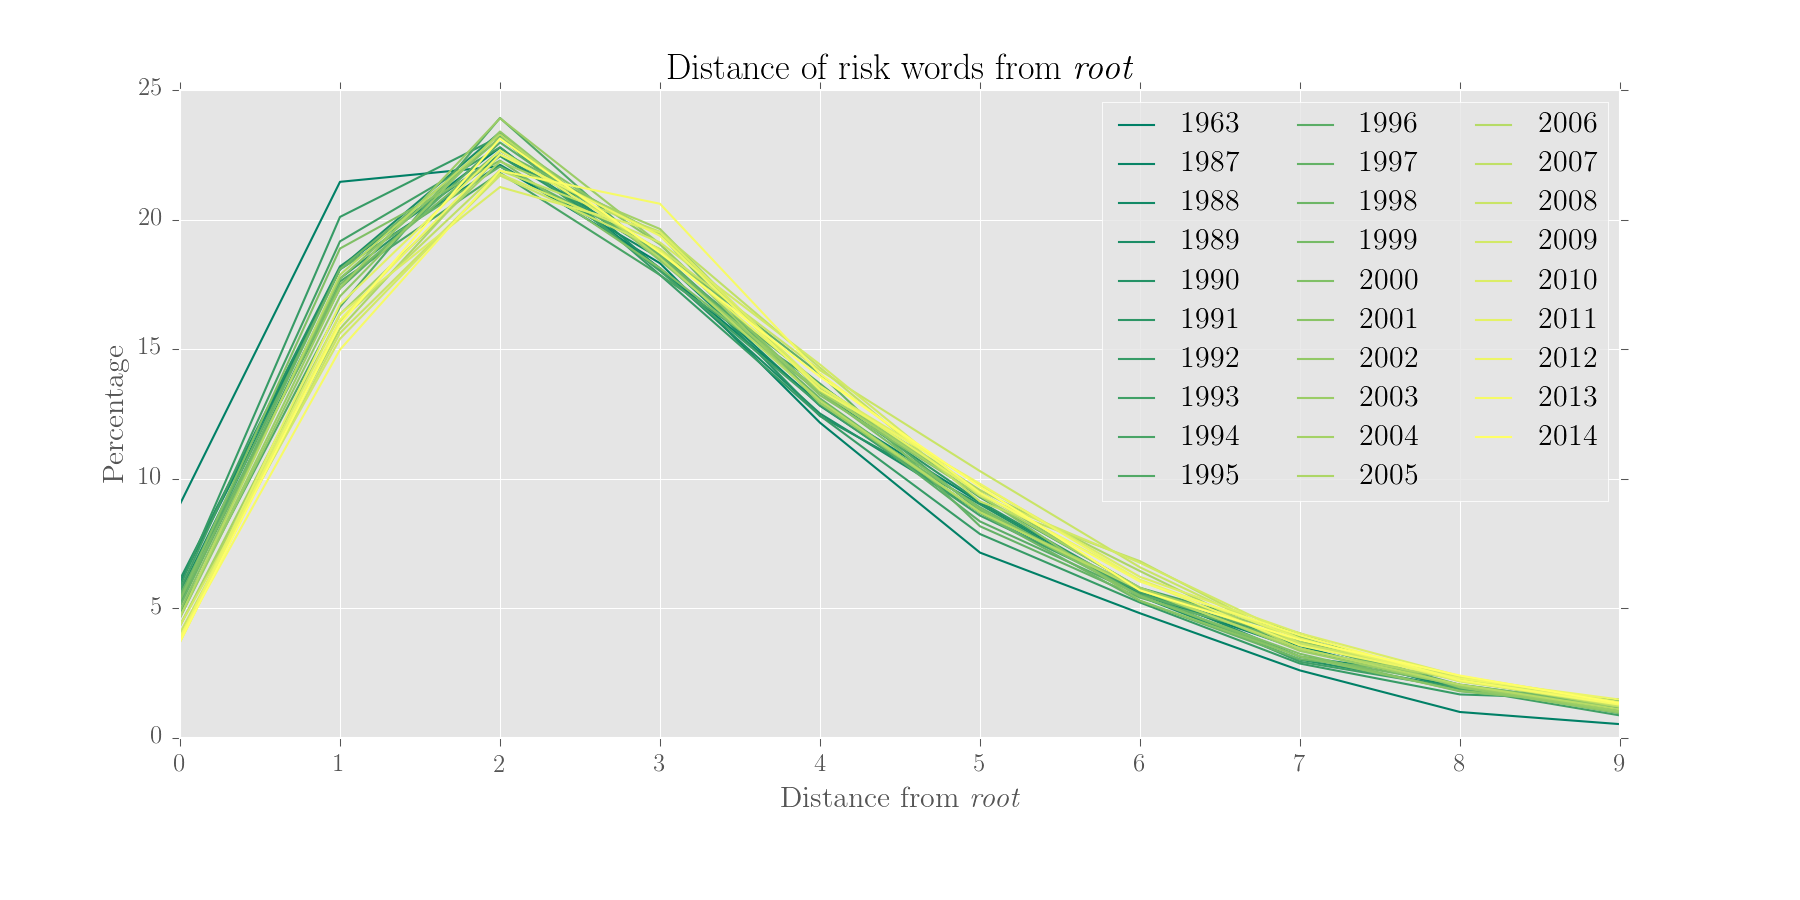
\includegraphics[width=1\textwidth]{../../images/distance-of-risk-words-from-root}

    ... looked promising, but seems to be a general phenomenon.
\end{frame}


\begin{frame}
    \frametitle{First investigation: key findings}
    
    \begin{itemize}
    \item Nominalisation and \emph{participantification}
    \begin{itemize}
        \item risking harm $\rightarrow$ risk assessment
        \item Meaning of risk expanding beyond the \emph{risk frame}
    \end{itemize}
    \item Risk words becoming more implicit
    \begin{itemize}
        \item Routinisation of the management of risk
        \item Risk as increasingly present, but decreasingly debated
    \end{itemize}
    \item More everyday exposure to risk, but less risking
    \begin{itemize}
        \item Neoliberal conceptualisations of agency: institutional expectation to take risk
        \item Reporting of `\emph{the scandal of not being in control}' \cite{beck_risk_1992}
    \end{itemize}
    \end{itemize}
\end{frame}

\begin{frame}\frametitle{Health risk}

\end{frame}

\begin{frame}\frametitle{Six newspapers}
\begin{itemize}
\item We've only just started interrogating the six newspaper corpus.
\item First, we'd like to check if the NYT findings are generalisable to other publications.
\item Would love help on dealing with the complexity of the data structure
\end{itemize}
\end{frame}

\begin{frame}\frametitle{Health risk}

\end{frame}

\begin{frame}\frametitle{Health risk}

\end{frame}


\begin{frame}\frametitle{Preliminary findings}
\begin{itemize}
    \item Most phenomena generalisable
    \item Some newspaper specific constructions: \emph{risk appetite} in the WSJ
    \item Fewer grammatical riskers, but risk characterising more participants and processes
    \item Hints of influence of newspaper's politican position
    \item 
\end{itemize}

\end{frame}







\begin{frame}
    \frametitle{Discussion of methodology}
    
    \begin{itemize}
    \item SFL proves a useful means of dividing up and investigating the behaviour of a given word
    \item SFL parsing is difficult, as is converting concepts from (esp. formal) grammars
    \item Difficult SF concepts: rank shift, grammatical metaphor, appraisal, process types \cite{yan_automatic_2014,costetchi_semantic_2013,heyvaert_nominalization_2003}
    \item That said, though theoretical orientations are different, much of the grammar (esp. at group\slash phrase levels) are similar

    \end{itemize}
\end{frame}

\begin{frame}
    \frametitle{Discussion: sociology and linguistics}
    
    Though SFL treats context as embedded in the lexicogrammar of texts, sociological theory can theorise the influence of salient events, people

    \begin{itemize}
        \item Did Chernobyl\slash Sept. 11 \emph{change} language use in the NYT?
    \end{itemize}

    Functional linguistic theory and corpus\slash computational linguistic provide sociology research with:

    \begin{itemize}
        \item Empiricism
        \item Reproducibility
    \end{itemize}
\end{frame}

\begin{frame}
    \frametitle{It's all open source}
    Data and tools are available for reuse:
    \begin{itemize}
    \item \url{https://www.github.com/interrogator/risk}
    \item \url{https://www.github.com/interrogator/corpkit}
    \end{itemize}
    Findings are presented dynamically in an IPython Notebook: 
    \begin{itemize}
    \item \url{http://git.io/vIM2W}
    \end{itemize}
    This slideshow:
    \begin{itemize}
    \item \url{http://git.io/vBfbw}
    \end{itemize}
\end{frame}

    \begin{frame}[t,allowframebreaks]
    \frametitle{References}
    \bibliographystyle{apacite}
    \bibliography{../report/references/references}
    \end{frame}
    
    \end{document}